\chapter{Analisis}
\label{chap:analisis}
Bab ini berisi analisis pemodelan properti kelas, analisis pemanfaatan pustaka Three.js, dan analisis penggunaan WebGL.

\section{Analisis Pemodelan Properti Kelas}
\label{sec:pemodelanproperti}
Pemodelan properti kelas merupakan proses dibuatnya masing-masing satuan properti yang dimiliki oleh kelas pada Fakultas Teknologi Informasi dan Sains. Pada proses pemodelan akan dilakukan pembentukan properti kelas pada editor hingga menyerupai bentuk asli dari properti yang sedang dimodelkan. Penulis memanfaatkan bantuan aplikasi Blender\footnote[1]{https://www.blender.org/} dalam melakukan pemodelan properti kelas. Aplikasi Blender (subbab ~\ref{sec:blender}) merupakan sebuah perangkat lunak untuk membangun grafika 3 dimensi. Terdapat 2 buah tahapan dalam memodelkan suatu bentuk properti, yaitu sebagai berikut:
\begin{itemize}
	\item {\bf Pembentukan model}, pada tahap ini dilakukan berbagai cara untuk memanipulasi bentuk model hingga bentuknya menyerupai properti yang asli. Dilakukan berbagai usaha untuk dapat menyerupai bentuk dari properti asli seperti {\it selecting, extruding, rotating, scaling, moving}, dan lain-lain. Pada gambar ~\ref{fig:modelling1} dapat dilihat proses pembentukan model untuk properti meja dosen.
	\item {\bf Pemetaan tekstur}, pada tahap ini dilakukan pemetaan permukaan objek ke gambar tekstur yang cocok dengan model tersebut. Setiap bagian permukaan dari model akan dibuka hingga menjadi satu permukaan datar. Kemudian permukaan datar tersebut akan ditempelkan kepada tekstur yang cocok dengan model tersebut. Pada gambar ~\ref{fig:uvwrap1} dapat dilihat proses pembukaan setiap permukaan dari model meja dosen hingga menjadi satu permukaan datar. Kemudian hasil akhirnya dapat dilihat pada gambar ~\ref{fig:modelwarna1}.
	\begin{figure}
		\centering
		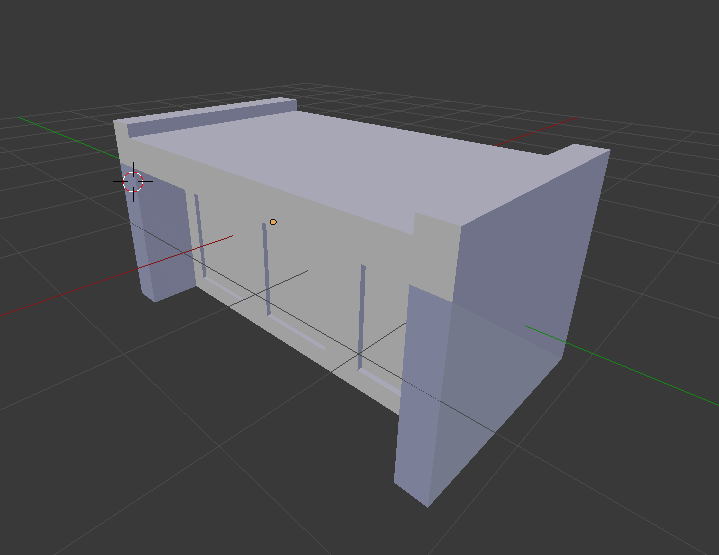
\includegraphics[scale=0.5]{modelling1}
		\caption{Meja sederhana yang selesai dibentuk namun belum diberi tekstur}
		\label{fig:modelling1}
	\end{figure}
	\begin{figure}
		\centering
		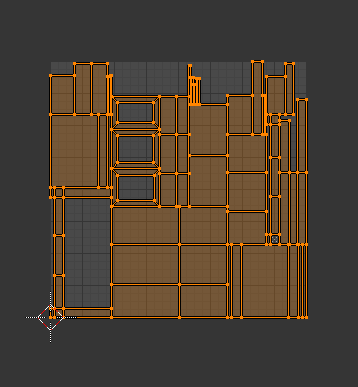
\includegraphics[scale=0.8]{uvwrap1}
		\caption{Pembukaan setiap bagian permukaan dari model meja dosen hingga menjadi satu permukaan datar}
		\label{fig:uvwrap1}
	\end{figure}
	\begin{figure}
		\centering
		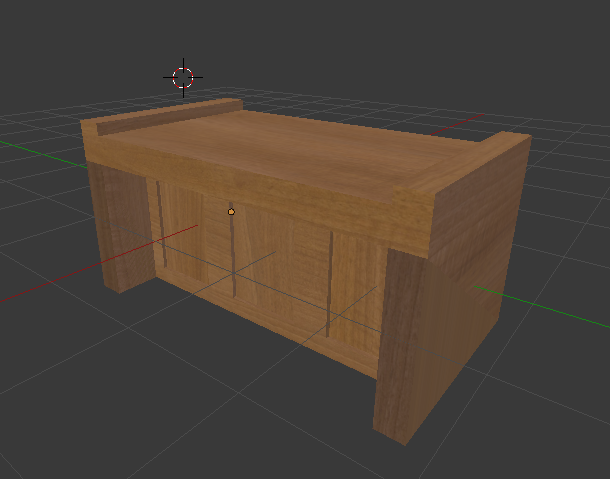
\includegraphics[scale=0.6]{modelwarna1}
		\caption{Hasil akhir pemodelan properti meja dosen}
		\label{fig:modelwarna1}
	\end{figure}
\end{itemize}

\section{Analisis pemanfaatan pustaka Three.js}
\label{sec:pemanfaatanthreejs}
Pada pengimplementasian Aplikasi Pratinjau 3 Dimensi Berbasis Web digunakan banyak fitur yang telah disediakan oleh pustaka Three.js. Berikut ini merupakan daftar fitur pustaka Three.js yang digunakan pada implementasi Aplikasi Pratinjau 3 Dimensi Berbasis Web:

\subsection{Panggung}
Panggung ({\it scene}) merupakan sebuah wadah untuk menempatkan sesuatu pada pustaka Three.js (subbab ~\ref{sec:objekumum}). {\it Scene} harus selalu diimplementasikan karena merupakan elemen dasar yang diperlukan pada representasi grafika 3 dimensi. Contoh penggunaan {\it Scene} pada implementasi Aplikasi Pratinjau 3 Dimensi Berbasis Web dengan latar warna putih dapat dilihat pada {\it listing} ~\ref{lst:scene}.
\begin{lstlisting}[caption={Contoh penggunaan {\it Scene}}, label={lst:scene},captionpos=b]
var scene = new THREE.Scene();
scene.background = new THREE.Color(constant.worldColor);
\end{lstlisting}

\subsection{Cahaya}
Pada dunia 3 dimensi dan khususnya pada pemanfaatan pustaka Three.js (subbab ~\ref{sec:objekumum}), telah disediakan berbagai macam cahaya untuk memberikan pencahayaan pada layar. Contoh cahaya yang disediakan oleh pustaka Three.js adalah {\it AmbientLight, DirectionalLight, Hemisphere Light, PointLight, RectAreaLight} dan {\it SpotLight}. Namun pada implementasi kelas Fakultas Teknologi Informasi dan Sains ke dalam model 3 dimensi tidak digunakan cahaya, hal tersebut terjadi karena telah digunakan material yang dapat terlihat meskipun tanpa ada cahaya pada panggung tersebut. Material tersebut adalah {\it MeshBasicMaterial}, sebuah material yang paling sederhana dan tidak memperhitungan cahaya.

\subsection{Warna}
Pada implementasi Aplikasi Pratinjau 3 Dimensi Berbasis Web digunakan pemanfaatan objek warna yang telah disediakan oleh pustaka Three.js yaitu {\it Color} (subbab ~\ref{sec:objekspesifik}). Objek warna ini kemudian digunakan untuk memberikan pewarnaan pada latar dunia 3 dimensi pada pemodelan aplikasi ini. Contoh penggunaan {\it Color} pada implementasi aplikasi ini dapat dilihat pada {\it listing} ~\ref{lst:color}
\begin{lstlisting}[caption={Contoh penggunaan {\it Color}}, label={lst:color},captionpos=b]
var scene = new THREE.Scene();
scene.background = new THREE.Color(constant.worldColor);
\end{lstlisting}

\subsection{Kamera}
Pada implementasi Aplikasi Pratinjau 3 Dimensi Berbasis Web digunakan {\it PerspectiveCamera} yang telah disediakan oleh pustaka Three.js (subbab ~\ref{sec:objekumum}). {\it PerspectiveCamera} merupakan kamera yang menggunakan proyeksi perspektif. Terdapat juga jenis kamera lain seperti {\it CubeCamera} dan {\it OrthographicCamera}, namun pada implementasi Aplikasi Pratinjau 3 Dimensi Berbasis Web yang digunakan adalah {\it PerspectiveCamera} karena lebih cocok dalam representasi yang menyerupai perspektif dunia nyata. Contoh penggunaan {\it PerspectiveCamera} pada implementasi Aplikasi Pratinjau 3 Dimensi Berbasis Web dengan pengaturan kamera dan posisi tertentu dapat dilihat pada {\it listing} ~\ref{lst:perspectiveCam}.
\begin{lstlisting}[caption={Contoh penggunaan {\it PerspectiveCamera}}, label={lst:perspectiveCam},captionpos=b]
var camera = new THREE.PerspectiveCamera(75, window.innerWidth/
window.innerHeight, 0.1, 100, 100);
camera.position.set(0, 10, 40);
\end{lstlisting}

\subsection{Kontrol Kamera}
Pada implementasi Aplikasi Pratinjau 3 Dimensi Berbasis Web digunakan sebuah objek untuk kontrol kamera yang telah disediakan oleh pustaka Three.js (subbab ~\ref{sec:objekspesifik}). Objek tersebut adalah {\it OrbitControls}, objek ini memungkinkan kamera untuk dapat mengorbit disekeliling target. Contoh penggunaan {\it OrbitControls} pada implementasi Aplikasi Pratinjau 3 Dimensi Berbasis Web dapat dilihat pada {\it listing} ~\ref{lst:orbitControls}.
\begin{lstlisting}[caption={Contoh penggunaan {\it OrbitControls}}, label={lst:orbitControls},captionpos=b]
var camera = new THREE.PerspectiveCamera(75, window.innerWidth/
window.innerHeight, 0.1, 100, 100);
controls = new THREE.OrbitControls(camera, renderer.domElement);
\end{lstlisting}

\subsection{Pembangun WebGL}
WebGLRenderer merupakan pembangun model 3 dimensi untuk ditampilkan ke layar (subbab ~\ref{sec:objekspesifik}). Fitur ini menyediakan tempat untuk membangun {\it Scene} dan berbagai hal 3 dimensi lainnya. Contoh penggunaan {\it WebGLRenderer} pada implementasi Aplikasi Pratinjau 3 Dimensi Berbasis Web dengan batasan area hanya pada elemen {\it canvas} dapat dilihat pada {\it listing} ~\ref{lst:webglRenderer}.
\begin{lstlisting}[caption={Contoh penggunaan {\it WebGLRenderer}}, label={lst:webglRenderer},captionpos=b]
var renderer = new THREE.WebGLRenderer(
{canvas: document.getElementById('canvas'), antialias: true});
\end{lstlisting}
	
\subsection{Pemuat}
Terdapat dua buah pemuat yang digunakan dalam implementasi Aplikasi Pratinjau 3 Dimensi Berbasis web. Berikut ini merupakan penjelasan untuk kedua pemuat tersebut:
\begin{itemize}
	\item {Pemuat JSON}
{\it JSONLoader} merupakan pemuat objek dalam bentuk JSON (JavaScript Object Notation). Pemuat ini mengubah format JSON menjadi objek yang dapat dibaca oleh pustaka Three.js (subbab ~\ref{sec:objekspesifik}). Pada implementasi Aplikasi Pratinjau 3 Dimensi Berbasis Web, {\it JSONLoader} digunakan untuk membaca model properti kelas yang sebelumnya telah disimpan dalam format JSON. Contoh penggunaan {\it JSONLoader} pada implementasi Aplikasi Pratinjau 3 Dimensi Berbasis Web pada implementasi aplikasi ini dapat dilihat pada {\it listing} ~\ref{lst:jsonLoader}.
\begin{lstlisting}[caption={Contoh penggunaan {\it JSONLoader}}, label={lst:jsonLoader},captionpos=b]
var loader = new THREE.JSONLoader();
var callbackProperty = function(geometry) {
	var texture = new THREE.TextureLoader().load(property.texture);
	var material = new THREE.MeshBasicMaterial( { map : texture } ); 
	var mesh = new THREE.Mesh(geometry, material);
	mesh.position.set(dx,dy,dz);
	mesh.scale.set(property.scale,property.scale,property.scale);
	mesh.rotation.y = property.rotation;
	scene.add(mesh);
};
loader.load(property.model, callbackProperty);
\end{lstlisting}

	\item {Pemuat Tekstur}
{\it TextureLoader} merupakan pemuat untuk gambar tekstur. Pada implementasi Aplikasi Pratinjau 3 Dimensi Berbasis Web, {\it TextureLoader} digunakan untuk memuat gambar tekstur yang kemudian akan digunakan untuk model properti kelas (subbab ~\ref{sec:objekspesifik}). Contoh penggunaan {\it TextureLoader} untuk tekstur suatu {\it mesh} yang akan ditambahkan ke {\it Scene} pada implementasi Aplikasi Pratinjau 3 Dimensi Berbasis Web pada implementasi aplikasi ini ada pada {\it listing} ~\ref{lst:texLoader}.
\begin{lstlisting}[caption={Contoh penggunaan {\it TextureLoader}}, label={lst:texLoader},captionpos=b]
var texture = new THREE.TextureLoader().load(property.texture);
var material = new THREE.MeshBasicMaterial( { map : texture } ); 
var mesh = new THREE.Mesh(geometry, material);
mesh.position.set(dx,dy,dz);
mesh.scale.set(property.scale,property.scale,property.scale);
mesh.rotation.y = property.rotation;
scene.add(mesh);
\end{lstlisting}
\end{itemize}

\subsection{Material}
Terdapat dua buah material yang digunakan dalam implementasi Aplikasi Pratinjau 3 Dimensi Berbasis web. Berikut ini merupakan penjelasan untuk kedua material tersebut:
\begin{itemize}
	\item {\it MeshBasicMaterial}
{\it MeshBasicMaterial} merupakan sebuah bahan untuk menggambar geometri dengan cara yang sederhana dan datar (subbab ~\ref{sec:objekspesifik}). Pada implementasi Aplikasi Pratinjau 3 Dimensi Berbasis Web, {\it MeshBasicMaterial} digunakan untuk geometri-geometri properti kelas. Contoh penggunaan {\it MeshBasicMaterial} untuk suatu {\it mesh} yang akan ditambahkan ke {\it Scene} pada implementasi Aplikasi Pratinjau 3 Dimensi Berbasis Web dapat dilihat pada {\it listing} ~\ref{lst:meshBasicMat}.
\begin{lstlisting}[caption={Contoh penggunaan {\it MeshBasicMaterial}}, label={lst:meshBasicMat},captionpos=b]
var texture = new THREE.TextureLoader().load(property.texture);
var material = new THREE.MeshBasicMaterial( { map : texture } ); 
var mesh = new THREE.Mesh(geometry, material);
mesh.position.set(dx,dy,dz);
mesh.scale.set(property.scale,property.scale,property.scale);
mesh.rotation.y = property.rotation;
scene.add(mesh);
\end{lstlisting}

	\item {\it MeshFaceMaterial}
{\it MeshFaceMaterial} merupakan sebuah wadah yang memungkinkan kita untuk menspesifikan material unik pada setiap permukaan geometri (subbab ~\ref{sec:objekspesifik}). Pada implementasi Aplikasi Pratinjau 3 Dimensi Berbasis Web, {\it MeshFaceMaterial} digunakan untuk representasi ruangan kelas. Contoh penggunaan {\it MeshFaceMaterial} untuk representasi kelas dapat dilihat pada {\it listing} ~\ref{lst:meshFaceMat}.
\begin{lstlisting}[caption={Contoh penggunaan {\it MeshFaceMaterial}}, label={lst:meshFaceMat},captionpos=b]
var material = new THREE.MeshFaceMaterial(cubeMaterials);
var cube = new THREE.Mesh(geometry, material);
cube.position.y = 9.05;
cube.name = 'room';
scene.add(cube);
\end{lstlisting}
\end{itemize}

\subsection{Jala}
Jala ({\it mesh}) merupakan sebuah bentuk representasi objek (subbab ~\ref{sec:objekspesifik}). Pada implementasi Aplikasi Pratinjau 3 Dimensi Berbasis Web, {\it Mesh} digunakan untuk objek properti kelas. Contoh penggunaan {\it Mesh} yang akan ditambahkan ke {\it Scene} pada implementasi Aplikasi Pratinjau 3 Dimensi Berbasis Web dapat dilihat pada listing ~\ref{lst:mesh}
\begin{lstlisting}[caption={Contoh penggunaan {\it Mesh}}, label={lst:mesh},captionpos=b]
var texture = new THREE.TextureLoader().load(property.texture);
var material = new THREE.MeshBasicMaterial( { map : texture } ); 
var mesh = new THREE.Mesh(geometry, material);
mesh.position.set(dx,dy,dz);
mesh.scale.set(property.scale,property.scale,property.scale);
mesh.rotation.y = property.rotation;
scene.add(mesh);
\end{lstlisting}

\subsection{Geometri}
\label{sec:analisisgeometri}
Pada implementasi Aplikasi Pratinjau 3 Dimensi Berbasis Web digunakan satu buat geometri sebagai representasi dari ruangan kelas di Fakultas Teknologi Informasi dan Sains, geometri tersebut merupakan {\it BoxGeometry}. {\it BoxGeometry} merupakan sebuah geometri yang berbentuk segi empat (subbab ~\ref{sec:objekumum}). Contoh penggunaan {\it BoxGeometry} sebagai kelas yang akan ditambahkan ke {\it Scene} pada implementasi Aplikasi Pratinjau 3 Dimensi Berbasis Web dapat dilihat pada {\it listing} ~\ref{lst:boxGeo}.
\begin{lstlisting}[caption={Contoh penggunaan {\it BoxGeometry}}, label={lst:boxGeo},captionpos=b]
var geometry = new THREE.BoxGeometry(length, width, height);
var material = new THREE.MeshFaceMaterial(cubeMaterials);
var cube = new THREE.Mesh(geometry, material);
cube.position.y = 9.05;
cube.name = 'room';
scene.add(cube);
\end{lstlisting}
Terdapat sedikit keterbatasan pada penggunaan {\it BoxGeometry} untuk representasi ruangan kelas Fakultas Teknologi Informasi dan Sains. Geometri ini hanya memiliki 6 buah permukaan standar seperti bentuk kubus pada umumnya. Sementara itu pada ruangan Fakultas Teknologi Informasi dan Sains, dinding ruangan terbagi menjadi dua warna. Sehingga dibutuhkan 10 permukaan dengan material berbeda untuk masing-masing permukaan tersebut. Sehingga untuk menangani permasalahan tersebut, dibuat kombinasi campuran warna tekstur yang sesuai untuk pasangan warna dinding yang akan digunakan pada ruangan kelas. Setiap tekstur tersebut akan memiliki dua buat warna, sehingga banyak permukaan yang akan digunakan tetap hanya 6 buah.
Solusi lain yang mungkin dapat digunakan adalah dengan menambahkan 4 buah {\it PlaneGeometry} pada masing-masing permukaan yang merepresentasikan dinding ruangan. {\it PlaneGeometry} merupakan geometri sederhana yang datar. Geometri ini dapat digunakan untuk menutupi setengah bagian permukaan dinding ruangan agar dapat diberikan warna tekstur lainnya, hal ini memungkinkan kita untuk membuat dua buah warna tekstur pada satu permukaan dinding ruangan. Namun solusi ini tidak diambil oleh penulis karena apabila solusi ini digunakan maka ada satu fitur pada {\it BoxGeometry} yang tidak dapat digunakan. Fitur tersebut merupakan penghilangan permukaan dinding yang menghadap ke kamera. Fitur ini sangat berguna untuk kemudahan perspektif pengguna saat melakukan rotasi ruangan pada saat melakukan proses pratinjau. Penambahan {\it PlaneGeometry} pada permukaan dinding ruangan akan mengganggu perspektif pengguna, karena pada saat dilakukan rotasi ruangan {\it PlaneGeometry} tidak akan menghilang dan menutupi bagian yang menghadap ke kamera. Oleh karena itu, solusi ini tidak diambil oleh penulis.

\subsection{Vektor 3 Dimensi}
Pada implementasi Aplikasi Pratinjau 3 Dimensi Berbasis Web digunakan vektor sebagai representasi titik target tempat kamera mengarah. Titik target ini memiliki masing-masing nilai koordinat untuk sumbu X, sumbu Y, dan juga sumbu Z. Vektor yang digunakan adalah {\it Vector3} yang telah disediakan oleh pustaka Three.js (subbab ~\ref{sec:objekspesifik}). Contoh penggunaan {\it Vector3} sebagai representasi titik target pada implementasi Aplikasi Pratinjau 3 Dimensi Berbasis Web dapat dilihat pada {\it listing} ~\ref{lst:vector}
\begin{lstlisting}[caption={Contoh penggunaan {\it Vector3}}, label={lst:vector},captionpos=b]
camera.position.set(0, 10, 0);
controls.minDistance = 5;
controls.maxDistance = 15;

controls.target = new THREE.Vector3(0, 10, 0);
\end{lstlisting}

\section{Analisis Penggunaan WebGL}
Pada pembuatan Aplikasi Pratinjau 3 Dimensi Berbasis Web tidak digunakan Application Programming Interface (API) WebGL secara langsung. Pemrograman dengan menggunakan API WebGL secara langsung akan menjadi proses yang sangat kompleks. Oleh karena itu digunakan pustaka Three.js yang didasari oleh fitur dari WebGL namun dengan penggunaan yang jauh lebih mudah tanpa harus mempelajari WebGL secara detail. Pustaka Three.js telah membungkus API yang disediakan oleh WebGL agar menjadi lebih mudah dan sederhana untuk digunakan. Oleh karena itu tidak terdapat banyak analisis pada bagian ini karena WebGL tidak digunakan secara langsung pada pembuatan skripsi ini. 










